\question
Для представленного графа и ДОПОЛНИТЕЛЬНОГО к нему определите:
\begin{enumerate}
\item есть ли в графе Эйлеров цикл или Эйлерова цепь? Если есть, то постройте по шагам алгоритма Флери цепь/цикл. Если нет, то обоснуйте отсутствие;
\item есть ли в графе Гамильтонов цикл, Гамильтонова цепь? Если есть, постройте по шагам алгоритма цепь/цикл. Если нет, то обоснуйте отсутствие (проверьте все теоремы);
\end{enumerate}
Дополнительно: преобразуйте граф, добавляя новые ребра и вершины, чтобы он был одновременно Гамильтоновым и Эйлеровым.
\begin{figure}[h]

\begin{minipage}[h]{0.55\linewidth}
\end{minipage}
\begin{minipage}[h]{0.45\linewidth}
\center{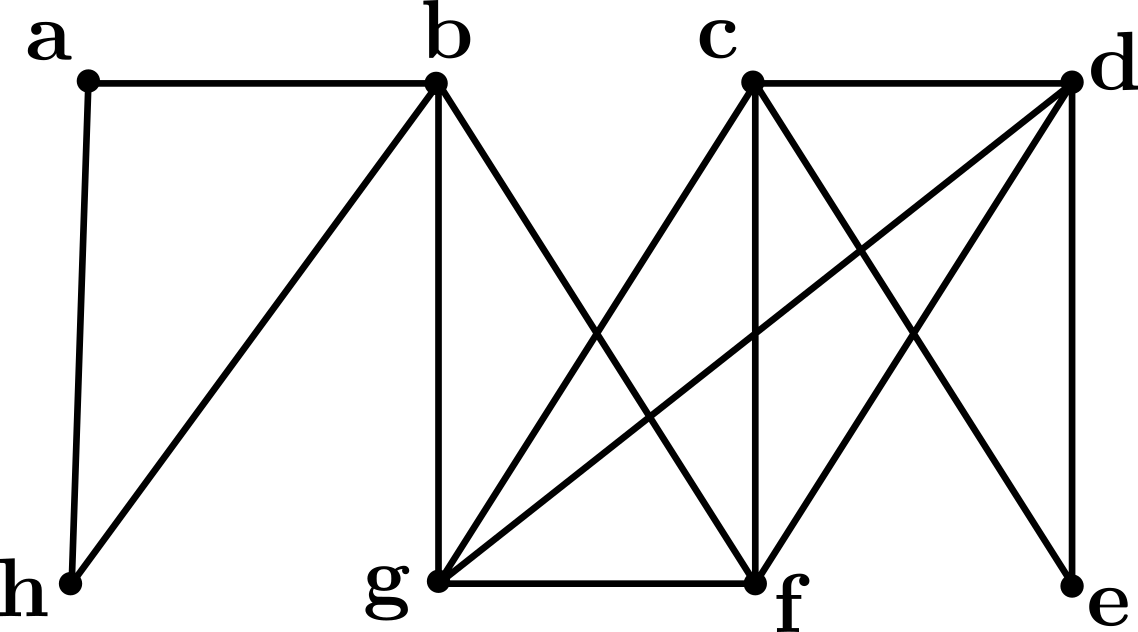
\includegraphics[width=0.6\textwidth]{pic/3.png}}
\end{minipage}
\end{figure}
